\subsection{Arrival: a common map and a known-input map have different optima}
\label{sec:arrival-optima-12}

The arrival comparison now separates three questions that were previously
left together. In normalized phase 9 coordinates let $P_s,P_a$ project onto
the symmetric and antisymmetric directions of the pairs $(0,5),(1,4),
(2,6),(3,8)$, and let $P_e$ be edge 7. The separated sector Grams are
\begin{equation}
 G_{42}=3P_s/5+P_e,\quad G_{33}=P_a/3,\quad
 G_{321}=2P_s/5+2P_a/3.
\end{equation}
The contact multipliers on the non-edge sectors are $47/45,17/15,14/15$.
With the stated complete flavor-factor alignment, the common-map cross
Gram is $C=c_sP_s+c_aP_a+P_e$, where
\begin{align}
 c_s&=\tfrac35\sqrt{47/45}+\tfrac25\sqrt{14/15},\\
 c_a&=\tfrac13\sqrt{17/15}+\tfrac23\sqrt{14/15}.
\end{align}
Sector Cauchy--Schwarz bounds every flavor-preserving overlap on a unit
antisymmetric pair by $c_a$. The displayed alignment attains this bound,
and $c_a<c_s<1$. Its minimax vector distance is therefore
$\sqrt{2-2c_a}$. For unchanged 14336 its $(P_s,P_a,P_e)$ weights are
$(2/9,2/3,1/9)$, giving the second row of
Table~\ref{tab:arrival-optima-12}.\samref{REF12_ONE}

\begin{table}[htbp]\centering\small
\caption{Coherent arrival errors in the normalized source norm.
Attainment requires the specified full-flavor orbital alignment.}
\begin{tabular}{p{1.65in}l}\toprule
Optimization domain & Enclosing distance\\\midrule
One map, worst source input&$[.0464409230216487,$\\
 &$ .0464409230216488]$\\
That map, unchanged 14336&$[.0400557228243080,$\\
 &$ .0400557228243081]$\\
Map chosen for known14336&$[.0396929079249281,$\\
 &$ .0396929079249282]$\\\bottomrule
\end{tabular}\label{tab:arrival-optima-12}
\end{table}

For the known-input optimum, maximize
$\sum_\lambda\sqrt{w_{{\rm sep},\lambda}w_{{\rm c},\lambda}}$ with
$w_{\rm sep}=(11/45,2/9,8/15)$ and
$w_{\rm c}=(169/675,34/135,112/225)$. The retained $321$ flavor factor is
common, so the required sector alignment is allowed in this stated
resource class. The squared errors of the last two rows differ by
$0.0000289339914409698435484\ldots>0$.

A deterministic channel with flavor-trivial ancillas preserves central
sector probabilities. Measuring those probabilities gives the distinct
mixed-output trace-distance obstruction
\begin{equation}
 \tfrac12\sum_\lambda|w_{{\rm c},\lambda}-w_{{\rm sep},\lambda}|
 =8/225.
\end{equation}
Trace distance here is half the trace norm; it is not the coherent vector
norm in the table. Flavor-carrying ancillary resources change the domain.
The coherent errors exceed the earlier $10^{-3}$ compiler allowance.
The conditional $15/17$ instrument and its retained failure branch remain
a separate arrival route.

\subsection{A sharp continuum loading floor at every finite duration}
\label{sec:loading-floor-12}

For the common shell spectrum, measure time by $\tau=R/c$ and let
$\mu=\dd s$ be a finite real signed measure of total mass one on $[0,T]$.
In the specified initially equilibrated energy-form sector the additional
coherent loading excess is
\begin{equation}
 \frac{E_{\rm res}}{D_{\rm jump}}
 =\iint\left(1-\frac{|t-u|}{2\tau}\right)_+
                      \mu(\dd t)\mu(\dd u).
\label{eq:loading-triangle-12}
\end{equation}
It follows from the full continuum density
$p_\tau(\omega)=2\tau\operatorname{sinc}^2(\tau\omega)/\pi$.
For a general incoming field the incoming energy and signed drive cross
term must also be retained; normalization alone does not imply this
initial-sector formula.\samref{REF12_CAR}

Put $a=2\tau$, $T/a=n+r$, $0\le r<1$, and
$m(x)=\mu((x-a,x])$. Box autocorrelation rewrites
\eqref{eq:loading-triangle-12} as $a^{-1}\int m(x)^2\dd x$.
For each residue $0<\theta<a$, the consecutive boxes partition the real
line and their signed masses sum to one. There are $n+2$ available boxes
for $0<\theta<ra$ and $n+1$ for $ra<\theta<a$. Cauchy--Schwarz on each
residue class, valid also for negative masses, proves
\begin{equation}
 \boxed{\frac{E_{\rm res}}{D_{\rm jump}}\ge
       q_*(T/a)=\frac{1-r}{n+1}+\frac r{n+2}>0.}
\label{eq:loading-floor-12}
\end{equation}
The exact deficit is the integral of squared departures of these box
masses from their uniform values. Thus this is a theorem for all finite
signed bounded-variation ramps, not only a numerical monotone optimizer.

For $0<r<1$, atoms at $ka$ and $(k+r)a$, $k=0,\ldots,n$, of weights
\begin{equation}
 A_k=\frac{n+1-k}{(n+1)(n+2)},\qquad
 B_k=\frac{k+1}{(n+1)(n+2)}
\end{equation}
make every residue load uniform and attain the bound. At integer duration
the coincident atoms merge into $n+1$ equal increments at spacing $2\tau$,
including the terminal increment. The continuum quadratic is strictly
positive on every nonzero compactly supported signed measure: its Fourier
transform cannot vanish on the positive-frequency continuum without
vanishing identically. Strict convexity therefore gives uniqueness.
Positive smooth ramps approach the atomic value as their rate caps
increase; one fixed finite rate cap does not generally attain it.

For comparison, a linear ramp has residual fraction
\begin{equation}
 q_{\rm lin}(T)=\begin{cases}
 1-T/(6\tau),&0\le T\le2\tau,\\
 2\tau/T-4\tau^2/(3T^2),&T\ge2\tau.
 \end{cases}
\end{equation}
Under $0\le s'\le M$ and $1/M\le T\le2\tau$, the sharp bounded-rate
value is $1-T/(4\tau)+1/(12\tau M)$. Finite selected optical modes can
cancel exactly while the continuum excess remains positive. Static
equilibrium shell displacement is also not a normal vacuum-Fock vector:
its infrared number integral diverges. Finite-time free-vacuum loading
is normal; the equilibrium construction must keep its energy-form-sector
qualification.

\begin{figure}[htbp]\centering
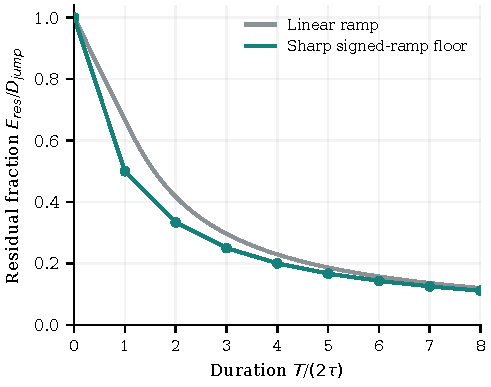
\includegraphics[width=\columnwidth]{refinement_20261112/figures/loading_floor.pdf}
\caption{Exact continuum residual fractions at equal duration. The lower
curve is the all-signed-ramp optimum; its atomic realization is distinct
from a bounded-rate physical controller. Both use the complete shell
spectrum and the stated incoming equilibrium sector.}
\label{fig:loading-floor-12}
\end{figure}

For an explicitly changed scalar reference $c-D$, the work identity is
\begin{equation}
 W=\Delta C+(c_1-D_1)-(c_0-D_0)+E_{\rm res}.
\end{equation}
Switching the coupling off with free zero and retaining a $+D$ scalar
baseline are different work conventions; neither changes the residual.
An incoming prepared cloud, conditional source measurement, controller
and reset require their own terms.

\subsection{Thirty exact carbon paths and the value of role information}
\label{sec:c12-paths-12}

The original count path has states $s=(a,b,c,d)$ for H1,H2,H3,He3,
seed $(6,0,0,0)$ and endpoint $(0,0,2,2)$. Its only actions are
\begin{align*}
 A:s&\mapsto(a-1,b+1,c,d),\\
 B:s&\mapsto(a,b-1,c+1,d),\\
 C:s&\mapsto(a-2,b,c,d+1),
\end{align*}
with nonnegative counts, $b+c\le2$ and $d\le2$. Each increments neutron
count by one. The admitted graph has 18 states and 30 six-action words.
The original full quadratic operand is
\begin{equation}
 Q=\begin{pmatrix}756&104&40&0\\104&2100&0&0\\
 40&0&756&40\\0&0&40&756\end{pmatrix}.
\end{equation}
In pair coordinates $a+4b$, form
\begin{equation}
 B_{a+4b,c+4d}=
 \frac{Q_{ac}Q_{bd}+\delta_{bd}Q_{ac}+\delta_{ac}Q_{bd}
                         +\delta_{ad}\delta_{bc}}{573049}.
\end{equation}
Average its 24 simultaneous role permutations to obtain $\bar B$.
For $u(s)=(a,b,c,2d)/6$, $v(s)=u(s)\otimes u(s)$, the full graph Gram
$K_{st}=v(s)^T\bar Bv(t)$ has rank ten. Its off-diagonal entries are
essential: deleting them changes even the canonical path cost.
\samref{REF12_FOUR}

Define edge variation $q_{st}=K_{ss}+K_{tt}-2K_{st}$ and signed work
$w_{st}=K_{tt}-K_{ss}$. Backward induction on neutron count proves the
Bellman recurrence $V(s)=\min_{s\to t}\{q_{st}+V(t)\}$, $V({\rm end})=0$.
Full enumeration gives the same answer,
\begin{equation}
 \min\sum q_{st}=225002149/139250907=1.6158038309941\ldots,
\end{equation}
a $7.327440840635\%$ reduction from canonical ABABCC's
$971170543/557003628=1.7435623291847\ldots$.
The literal canonical value is distinguished from the different
\texttt{reference\_energy\_profiles.current} field in the old prose.
Every path has the same signed endpoint work
$-264142984/139250907$. Minimum gross positive work is
$66534041/557003628$, while minimum storage is
$124789553/61889292$. All 30 mean-reference paths need zero ideal
reversible initial capital. These objectives have different minimizers.

The variation minimizers are AABCBC, AABCCB, AACBBC and AACBCB. CCABAB
minimizes gross positive work; CCAABB and CCABAB minimize storage.
The complete four-tuple Pareto frontier and all 30 exact paths are retained
in the source evidence; Figure~\ref{fig:c12-paths-12} shows all paths.

For the original 24 role assignments, optimizing after role information
lowers mean variation to $3476627797/2228014512$. The information value is
$13711843/247557168=0.05538859210087587\ldots$. Exhausting all one- and
two-word policies proves they cannot realize every rolewise minimum.
The unique three-word cover is AABCBC, AACBCB, ACBABC, with disjoint
fibers of sizes $6,12,6$. Thus exactly three decisions suffice for this
task. Its uniform-policy record has entropy $3\log2/2$; no globally
minimum-entropy policy theorem is asserted. Sensing, feedback, field
changes, failed contacts, clock, coherent storage and reset are unpriced.
The gain is in the specified quadratic source variation.

\begin{figure}[htbp]\centering
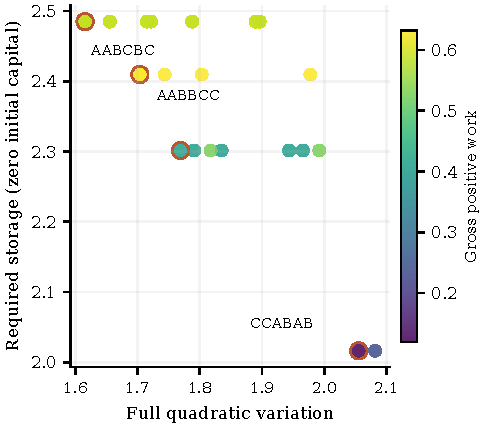
\includegraphics[width=\columnwidth]{refinement_20261112/figures/c12_paths.pdf}
\caption{All 30 admitted count paths on their complete source Gram.
Color gives gross positive work; outlined points lie on the joint
variation/work/storage frontier. Coincident objective tuples share points.
Data are exact rational source values, displayed as decimals.}
\label{fig:c12-paths-12}
\end{figure}

\subsection{Marked contacts, finite hazard and the held crossing variance}
\label{sec:contact-rice-12}

An isolated frozen eligible crossing with full-field acceptance $a$ has
column generator
\begin{equation}
 A=\begin{pmatrix}-a&1-a\\a&-(1-a)\end{pmatrix},\qquad A^2=-A.
\end{equation}
Consequently $e^{\lambda A}=I+(1-e^{-\lambda})A$.
One consumed timestamp and one uniform 48-label attempt instead gives
$I+A/48$. The matching isolated depth is $\lambda=\log(48/47)$,
not $1/48$. At the reachable $a=1/4$, the latter depth transfers
$0.005154454667189959\ldots$ rather than $1/192$.
This exact local mismatch leaves the separately constructed weak boundary
process intact. A global thin-layer limit must additionally pay freezing
error, post-jump eligibility and ordering at repeated/coincident surfaces.
\samref{REF12_FOUR}

The original centered held Gaussian process has normalized covariance
\begin{equation}
 r(h)=\begin{cases}
 1-3h^2/8+3|h|^3/32,&|h|\le2,\\
 (4-|h|)^3/32,&2\le|h|\le4,\\
 0,&|h|\ge4.
 \end{cases}
\end{equation}
It follows by autocorrelating the triangular Brownian-convolution kernel;
$-r''(0)=3/4$ and mean crossing rate is $\sqrt3/(2\pi)$ in unit-radius
time. If $r(h)=1-ah^2+b|h|^3+O(h^4)$, the derivative covariance conditioned
on two equal levels is
$2bh\left(\begin{smallmatrix}2&-1\\-1&2\end{smallmatrix}\right)+O(h^2)$.
Its velocity correlation tends to $-1/2$ and cancels the apparent
$h^{-1}$ singularity in the joint position density. The Rice pair density
has finite diagonal
\begin{equation}
 R_u(0+)=\left(\frac3{8\pi^2}+\frac{\sqrt3}{48\pi}\right)
                    e^{-u^2/2}/\tau^2.
\end{equation}
A $C^1$ modification, bounded one-time Gaussian density and a mesh
argument exclude level tangencies. The two-time coarea formula followed
by monotone convergence then proves a finite held second moment.

At zero level, pair excess is exactly zero beyond $4\tau$. Directed
integration of the factored nonsingular Rice density therefore gives
\begin{align}
 \Var N_T&=cT/\tau+b_0,\qquad T\ge4\tau,\\
 c&\in[.18892416368715884176181444213,\notag\\
     &\hspace{1.6em}.18892416368715884176181444214],\notag\\
 b_0&\in[.06022430801813990085076003477,\notag\\
     &\hspace{1.6em}.06022430801813990085076003478].\notag
\end{align}
In particular, at $\tau=1$,
\begin{equation}
\begin{split}
 \Var N_{16}\in[&3.08301092701268136903979110891,\\
               &3.08301092701268136903979110893].
\end{split}
\end{equation}
The affine law is exact on this held domain, not a Poisson approximation
or a fitted large-time slope. Endogenous/Palm weighting remains separate:
an $L^2$ change-of-law density would require a held fourth count moment
to infer the corresponding endogenous second moment. The held second
moment and almost-sure nonexplosion do not supply that missing premise.

\begin{figure}[htbp]\centering
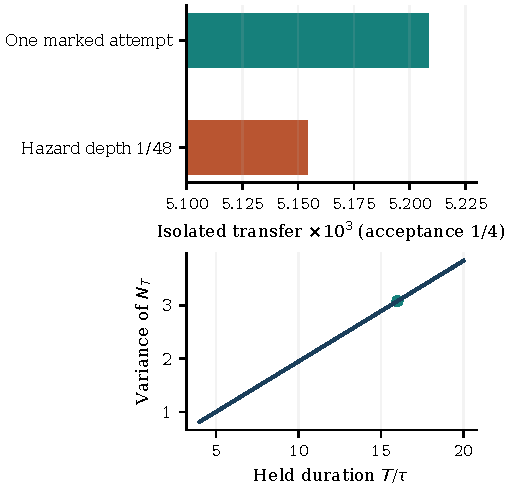
\includegraphics[width=\columnwidth]{refinement_20261112/figures/contact_variance.pdf}
\caption{Two distinct contact-law results. Above: the isolated finite-depth transfer differs from a consumed marked attempt. Below: the exactly affine centered held crossing variance for $T\ge4\tau$. No endogenous or Poisson count law is inferred.}
\label{fig:contact-variance-12}
\end{figure}
